\documentclass[12pt,titlepage]{article}

\usepackage{amsmath}
\usepackage{aas_macros}
\usepackage{rotating}
\usepackage{xspace}
\usepackage{booktabs}
\usepackage{array}
\usepackage{multirow}
\usepackage{color}
\usepackage{listings}
\usepackage{caption}
\usepackage[colorlinks=true,linkcolor=blue,urlcolor=blue]{hyperref}
\usepackage{dirtree}
\usepackage{adjustbox}
\usepackage{bytefield}
\usepackage{chngcntr}

%% stdsection is the old section -> no new page
%% section produces a new page before a new section
\let\stdsection\section
\renewcommand\section{\newpage\stdsection}

%% Some of the short-cuts I use
\newcommand{\rmax}{\ensuremath{{r_{max}}}\xspace}
\newcommand{\xir}{\ensuremath{{\xi(r)}}\xspace}
\newcommand{\wprp}{\ensuremath{{w_p(r_p)}}\xspace}
\newcommand{\xirppi}{\ensuremath{{\xi(r_p,\pi)}}\xspace}
\newcommand{\todo}[1]{\marginpar{TODO}{\color{red}#1}}
\newcommand{\clang}{{\texttt{clang}}\xspace}
\newcommand{\icc}{{\texttt{icc}}\xspace}
\newcommand{\gcc}{{\texttt{gcc}}\xspace}

%% Fill out space with dots
\newcommand\DotFill{\leavevmode\xleaders\hbox{.}\hfill\kern0pt}

%% New column type in tables
\newcolumntype{M}[1]{>{\raggedright\arraybackslash}m{#1}}

%% Code paper - so there are lots of code listings
\lstset{
  language=C,                % choose the language of the code
  basicstyle=\ttfamily,      % sets font
  numbers=none,                   % where to put the line-numbers
  numberstyle=\small, 
  stepnumber=1,                   % the step between two line-numbers.
  numbersep=10pt,                  % how far the line-numbers are from the code
  backgroundcolor=\color{white},  % choose the background color. You must add \usepackage{color}
  showspaces=false,               % show spaces adding particular underscores
  showstringspaces=false,         % underline spaces within strings
  showtabs=false,                 % show tabs within strings adding particular underscores
  tabsize=2,                      % sets default tabsize to 2 spaces
  captionpos=b,                   % sets the caption-position to bottom
  breaklines=true,                % sets automatic line breaking
  breakatwhitespace=true,         % sets if automatic breaks should only happen at whitespace
}
%% Change the listings counter to show Section number + listings number (rather than just the listings number)
\AtBeginDocument{\counterwithin{lstlisting}{section}}

%% I dislike paragraph indents
\setlength{\parindent}{0pt}

\begin{document}

\title{User Guide for Corrfunc}
%% Abuse the author macro to show all the info I want.
\author{Manodeep Sinha, \\
  Department of Physics \& Astronomy,\\
  Vanderbilt University,\\
  Nashville, TN 37235.\\
  \href{mailto:manodeep@gmail.com}{\texttt{manodeep@gmail.com}}
}

\maketitle 

\pagenumbering{Roman}
\tableofcontents
\pagenumbering{arabic}

\section{Introduction}
Correlation functions are a statistical measure of a density field and are widely used in large-scale structure formation. Generally, 
the measurements are done {\em once}\footnote{which is why I have not bothered with releasing the codes to measure correlation 
functions on data} on survey data and compared with model predictions in a Monte-Carlo Markov Chain. As such, the 
correlation functions have to be measured repeatedly during an MCMC. The codes presented here are meant to cover the typical scenarios 
of measuring correlation functions in theory-land. The primary consideration in writing these codes is speed\footnotemark -- the codes 
presented here should outperform any other CPU based correlation functions codes by a wide-margin. 

\footnotetext{The secondary consideration was maintainability and ease of use for others. I have versions of these codes that are 
even faster but are potentially gibberish for anyone other than me!}

\section{Installation}
The only requirements for the code to install is a valid C compiler, with OpenMP support. The AVX
instruction set can only be used for CPU's later than 2011 (Intel Sandy Bridge/ AMD Bulldozer or later). 

\subsection{Getting the Source}
You can obtain the source in two ways: i) Clone the mercurial repo (\texttt{hg clone} \url{https://bitbucket.org/manodeep/corrfunc/}) 
or ii) Download the tar archive (\href{https://bitbucket.org/manodeep/corrfunc/downloads/corrfunc.1.0.0.tar.gz}{corrfunc.\$MAJOR.0.\$MINOR.tar.gz}) and 
unpack it in the directory where you wish to keep the files (\texttt{tar xvzf corrfunc.\$MAJOR.0.\$MINOR.tar.gz}). Here, \$MAJOR and \$MINOR
refer to the major and minor release versions (current \$MAJOR=1, \$MINOR=0). I will only change the \$MAJOR version if the API breaks. 

The directory structure for the code looks like this:
\dirtree{%
.1 corrfunc.
.2 paper.
.2 xi\_theory.
.3 benchmarks\DotFill
  \begin{minipage}[t]{8cm}
    IDL scripts to run benchmarks{.} 
  \end{minipage}.
.3 bin\DotFill 
  \begin{minipage}[t]{8cm}
    Will be created to copy executable files when you run `make install'{.} 
  \end{minipage}.
.3 examples\DotFill 
  \begin{minipage}[t]{8cm}
    Source files for example C bindings using the static libraries{.} 
  \end{minipage}.
.3 include\DotFill 
  \begin{minipage}[t]{8cm}
    Header files for static libraries{.} 
  \end{minipage}.
.3 io\DotFill 
  \begin{minipage}[t]{8cm}
    Source files for reading in data{.} 
  \end{minipage}.
.3 lib\DotFill 
  \begin{minipage}[t]{8cm}
    Will be created to copy static libraries and python library after you run `make'{.} 
  \end{minipage}.
.3 python\_bindings\DotFill 
  \begin{minipage}[t]{8cm}
    Source files to generate python bindings{.} 
  \end{minipage}.
.3 tests\DotFill 
  \begin{minipage}[t]{8cm}
    Correct outputs for tests{.}
  \end{minipage}.
.4 data\DotFill 
  \begin{minipage}[t]{8cm}
    Mock galaxy catalogs for tests{.} 
  \end{minipage}.
.3 utils\DotFill 
  \begin{minipage}[t]{8cm}
    Source files for creating 3-D grid and helper routines{.} 
  \end{minipage}.
.3 wp\DotFill 
  \begin{minipage}[t]{8cm}
    Source files for $w_p(r_p)${.} 
  \end{minipage}.
.3 xi\_of\_r\DotFill 
  \begin{minipage}[t]{8cm}
    Source files for $\xi(r)${.} 
  \end{minipage}.
.3 xi\_rp\_pi\DotFill 
  \begin{minipage}[t]{8cm}
    Source files for $\xi(r_p,\pi)${.} 
  \end{minipage}.
}

\subsection{Code Options}
There are a few code options that control both the Science case and the code compilation. All of these 
options are located in `common.mk' in the base directory (`corrfunc'). Edit the first few lines to set these 
options (see Table.~\ref{table:options} for details) :
\begin{itemize}
\item Science options -- PERIODIC, OUTPUT\_RPAVG
\item Code options -- DOUBLE\_PREC, USE\_AVX and USE\_OMP
\end{itemize}

\begin{table}
\begin{center}
\begin{adjustbox}{max width=\textwidth}
\begin{tabular}{ccccM{4in}} 
\toprule
\multicolumn{1}{c}{\textbf{Option Type}}   &
\multicolumn{1}{c}{\textbf{Option Name}}   &
\multicolumn{1}{c}{\textbf{Default State}} &
\multicolumn{1}{c}{\textbf{Requires}}      &
\multicolumn{1}{c}{\textbf{Notes}}      \\
\midrule
                 & PERIODIC            & Enabled  & None            & Enables periodic boundary conditions. \\
\textbf{Science} & OUTPUT\_RPAVG       & Disabled & DOUBLE\_PREC    & Outputs the average pair-separation in each bin. \xir and \wprp can be slower by more than $2\times$, \xirppi is less affected. \\
\midrule
                 & DOUBLE\_PREC        & Disabled & None                               & Computations are done using double precision. Slower and requires more RAM. \\
\textbf{Code}    & USE\_AVX            & Enabled  & CPU and compiler with AVX support  & CPUs later than 2011 have AVX support. Code will run much faster with this option. \\
                 & USE\_OMP            & Enabled  & OpenMP capable compiler            & Since \clang does not support OpenMP yet, \texttt{common.mk} will stop compilation with \clang when this flag is enabled. \\
\bottomrule
\end{tabular}
\end{adjustbox}
\end{center}
\caption{\footnotesize List of compilations options, what the options mean and their dependencies for the codes. }
\label{table:options}
\end{table}
Depending on your Science use-case and the cpu/compiler, you will want to set the different options. Once you set those options, you should set the 
C compiler, CC (available options are \icc, \gcc, \clang). Once you have set the compiler, installing should be as simple as typing `make' and 
`make install' in the \texttt{xi\_theory} directory. All the libraries are intentionally chosen to be \texttt{static} libraries just to avoid 
any path conflicts. However, on MAC OSX, you may have to do more to get the library to work -- so I have outlined some of the scenarios in 
Section~\ref{section:mac}. 
\subsection{Linux}
If the installation went well, you should have an executable called \texttt{run\_correlations} in the \texttt{examples} directory. Type \texttt{./run\_correlations} 
in the \texttt{examples} directory and you should see the code in action. The C source file \texttt{run\_correlations.c} also serves as an example to 
use the \xir, \xirppi and \wprp libraries in C. 

\subsection{Mac OSX}\label{section:mac}
There can be two issues on MACs. One is that the default \gcc assembler supplied by \texttt{XCode} or \texttt{macports} is too old and does not support AVX instructions 
even when the CPU does. One way to get around this is by using the \clang assembler even when compiling with \gcc. The easiest way to do it is by replacing the 
default assembler with the \texttt{as} script in the \texttt{paper} directory (taken from \href{https://gist.github.com/ancapdev/8059572}{this url}). Copy this
\texttt{as} script to the appropriate directory (\texttt{/opt/local/bin/} for me since I use \texttt{macports} \gcc on my laptop).

Another problem might come with running the python example codes in the \texttt{python\_bindings} directory. If you get an error message:
\begin{itemize} 
\item \texttt{Fatal Python error: PyThreadState\_Get: no current thread} 
\end{itemize}
when you run \texttt{python call\_correlation\_functions.py}, then the following 
steps might fix the problem (these are also noted in the FAQ). This error occurs when the python library used at compile time is not the same 
as the runtime python library. In all cases that I have seen, this error occurs when using the \texttt{conda} package manager for python\footnote{This 
behaviour is by design according to \texttt{conda}}. 
\begin{itemize}

\item Change the relative path for the shared python library \_countpairs.so. You can change the relative path by issuing the command: \\
{\scriptsize\texttt{install\_name\_tool -change libpython2.7.dylib  \`{}python-config --prefix\`{}/lib/libpython2.7.dylib \_countpairs.so}}

\item Add to the fallback library path environment variable. \\
{\scriptsize\texttt{export DYLD\_FALLBACK\_LIBRARY\_PATH=\`{}python-config --prefix\`{}/lib:\$DYLD\_FALLBACK\_LIBRARY\_PATH}}

\item If both of the above methods fail, then create a symbolic link \\
{\scriptsize\texttt{ln -s \`{}python-config --prefix\`{}/lib/libpython2.7.dylib}}
\end{itemize}
If all went well, then you should be able to run the \texttt{run\_correlations} code in the \texttt{examples} directory as well as execute \texttt{python call\_correlation\_functions.py} 
in the \texttt{python\_bindings} directory. In all of the above examples, I have assumed that the relevant python library is \texttt{libpython2.7.dylib} (the default 
under \texttt{conda}) -- you may have to replace it with your python library version.

\section{Running the Codes}
\subsection{Input Files}
The codes currently can handle these types of input data files:
\begin{itemize}
\item \texttt{ascii} -- White-space separated columns, format code is `a'.
\item \texttt{csv}   -- Comma-separated values, format code is `c'.
\item \texttt{fast-food} -- Fast-food, fortran binary format, format code is `f'.
The fast-food file format is described in detail in Section~\ref{section:fastfood}.
\end{itemize}
For the \texttt{ascii} and \texttt{csv} files, the code reads in the first three columns as the co-moving \texttt{X/Y/Z} arrays. Note, that more columns 
can be present but the code will ignore those columns. 

\subsubsection{The fast-food file format}\label{section:fastfood}
The fast-food format is a fortran binary format -- all fields are surrounded with 4 bytes padding. These value of these padding bytes 
is the number of bytes of data contained in between the padding bytes. For example, to write out \texttt{20 bytes of data} in 
a fast-food file format would require a total of $4+20+4=28$ bytes. The first and last 4 bytes of the file will contain the value $20$ -- 
showing that 20 bytes of real data are contained in between the two paddings. 

\flushleft The \texttt{fast-food} file consists of a header:
\begin{lstlisting}[language=C,numbers=none]
int idat[5];
float fdat[9];
float znow;
\end{lstlisting}
For the purposes of these correlation function codes, the only useful quantity is \texttt{idat[1]} which contains \texttt{N} -- the number of particles 
in the data file. 

\vspace{0.2in}
%% \begin{enumerate}
%% \item
\begin{bytefield}{28}
  \bitheader{0-27} \\
  \bitbox{4}{20} & \bitbox{4}{Int} & \bitbox{4}{\textcolor{red}{\texttt{N}}} \bitbox{12}{3 Integers}& \bitbox{4}{20}\\
\end{bytefield}\\
%% \item
%% \begin{bytefield}{44}
%%   \bitheader{0-43} \\
%%  \bitbox{4}{36} & \bitbox{36}{9 Floats} & \bitbox{4}{36} \\
%% \end{bytefield}
%% %% \item
%% \begin{bytefield}{12}
%%   \bitheader{0-11} \\
%%   \bitbox{4}{4} & \bitbox{4}{Float} & \bitbox{4}{4}\\
%% \end{bytefield}
%% \end{enumerate}
The next 56 bytes contain two other fields (10 floats + 4 padding bytes of 4 bytes each) and their corresponding paddings. Since these bytes do not contain any data 
that are useful in the context of these codes we will skip over the contents of these bytes. In \texttt{io.c}, I actually \texttt{fseek} over these bytes. 

\flushleft After this header, the actual \texttt{X/Y/Z} values are stored. The first 4 bytes after the header contains \texttt{N*4, for float precision} or \texttt{N*8, for 
double precision} where \texttt{N=idat[1]}, is the number of particles in the file. After all the \texttt{X} values there will be another 4 bytes containing 
\texttt{N*4} or \texttt{N*8}. {\em Note, that even when the \texttt{X/Y/Z} arrays are written out in double-precision, the padding is still 4 bytes.}
\begin{minipage}[t]{\textwidth}
\centerline{\underline{\bfseries Byte-structure of the X/Y/Z arrays in a fast-food file}}
\vspace{0.2in}
\begin{minipage}[t]{0.5\textwidth}
\centering
\textbf{floats}\\[3ex]
\begin{bytefield}{4}
  \bitheader{0-3} \\
  \bitbox{4}{\texttt{N*4}} \\
  \wordbox{1}{X[0]} \\
  \wordbox{1}{X[1]} \\
  \wordbox[]{1}{$\vdots$} \\[1ex]
  \wordbox{1}{X[N-1]} \\
  \bitbox{4}{\texttt{N*4}}
\end{bytefield} 
\end{minipage}%
\begin{minipage}[t]{0.5\textwidth}
\centering
\textbf{doubles}\\[3ex]
\begin{bytefield}{8}
  \bitheader{0-7} \\
  \bitbox{4}{\texttt{N*8}} \\
  \wordbox{1}{X[0]} \\
  \wordbox{1}{X[1]} \\
  \wordbox[]{1}{$\vdots$} \\[1ex]
  \wordbox{1}{X[N-1]} \\
  \bitbox{4}{\texttt{N*8}}
\end{bytefield}
\end{minipage}
\end{minipage}
\subsection{Specifying the radial bins}\label{section:bins}
The codes were intentionaly designed to read in a set of (somewhat) arbitrary\footnote{I assume bins are non-overlapping} set of bin specifications from a file. This way, you can specify disjoint bin-edges as well as 
use $0.0$ as a bin edge (which would be impossible if $\log$ bins are assumed). The bins are to be specified in a (white-space separated) text file in this manner:
\begin{verbatim}
r_low[0]  r_high[0]
r_low[1]  r_high[1]
.
.
.
r_low[nbins-1]  r_high[nbins-1]
\end{verbatim}
where, \texttt{r\_low[i]} and \texttt{r\_high[i]} are the left and right edges of the \texttt{i}'th bin respectively. The text files should contains as many lines as the number of 
bins desired. The \texttt{logbins} executable can be used to create such a text file containing $\log$ bins. The syntax for running \texttt{logbins} is:
\begin{lstlisting}[language=sh,numbers=none]
./logbins <rmin> <rmax> <nbins>   > <text filename>
\end{lstlisting}
An example of such a file with radial bins is the file \texttt{bins} in the \texttt{tests} directory. 

{\em Note, all of the three codes print the correlation function to \texttt{stdout} -- so be sure to redirect \texttt{stdout} to an output file. }

\subsection{Running \texorpdfstring{\xir}{xi(r)}}
To run the correlation function in 3-D, you will need to run the executable \texttt{DD} from either the \texttt{bin} or \texttt{xi\_of\_r} directory. The inputs 
to \texttt{DD} are:
\begin{itemize}
\item \texttt{file1}   -- the file name for the first file.
\item \texttt{format1} -- the file format for the first file.
\item \texttt{file2}   -- the file name for the second file.
\item \texttt{format2} -- the file format for the second file.
\item \texttt{binfile} -- the file name for the file containing the bins (see Section~\ref{section:bins})
\item \texttt{nthreads} -- the number of OpenMP threads to use (only required when the Makefile option USE\_OMP is enabled)
\end{itemize}
Thus, the code can compute an auto-correlation (when \texttt{file1,format1} and \texttt{file2,format2} are identical) or a cross-correlation (when \texttt{file1} and \texttt{file2} are different). Out of the box, 
some sample \texttt{DD} call directory) can be:
\begin{itemize}
\item auto-correlation --  {\scriptsize \texttt{./DD  ../tests/data/gals\_Mr19.ff f ../tests/data/gals\_Mr19.ff f ../tests/bins 4 > Mr19\_output.DD}}
\item cross-correlation -- {\scriptsize \texttt{./DD ../tests/data/cmassmock\_Zspace.ff f ../tests/data/random\_Zspace.ff f ../tests/bins 4 > cmass\_output.DR}}
\end{itemize}
The output (printed to stdout) has \texttt{nbins} columns \texttt{<Npairs> <rpavg> <rmin> <rmax>}, where the \texttt{<rpavg>} column contains \texttt{0.0} unless the 
Makefile option OUTPUT\_RPAVG has been enabled. Here, each line of the output represents the \texttt{i}'th radial bin. 

\subsection{Running \texorpdfstring{\xirppi}{xi(rp,pi)}}
To run the correlation function in 2-D for \xirppi, you will need to run the executable \texttt{DDrppi} from either the \texttt{bin} or \texttt{xi\_rp\_pi} directory. The inputs 
to \texttt{DDrppi} are:
\begin{itemize}
\item \texttt{file1}   -- the file name for the first file.
\item \texttt{format1} -- the file format for the first file.
\item \texttt{file2}   -- the file name for the second file.
\item \texttt{format2} -- the file format for the second file.
\item \texttt{binfile} -- the file name for the file containing the bins (see Section~\ref{section:bins})
\item \texttt{pimax}   -- the maximum distance to consider in the $\pi$ direction. The code uses \texttt{Z} axis as the $\pi$ (line-of-sight) direction. 
\item \texttt{nthreads} -- the number of OpenMP threads to use (only required when the Makefile option USE\_OMP is enabled)
\end{itemize}
Thus, the code can compute an auto-correlation (when \texttt{file1,format1} and \texttt{file2,format2} are identical) or a cross-correlation (when \texttt{file1} and \texttt{file2} are different). Out of the box, 
some sample \texttt{DDrppi} call directory) can be:
\begin{itemize}
\item auto-correlation --  {\scriptsize \texttt{./DDrppi  ../tests/data/gals\_Mr19.ff f ../tests/data/gals\_Mr19.ff f ../tests/bins 40.0 4 > Mr19\_output\_rppi.DD}}
\item cross-correlation -- {\scriptsize \texttt{./DDrppi ../tests/data/cmassmock\_Zspace.ff f ../tests/data/random\_Zspace.ff f ../tests/bins 80.0 4 > cmass\_output\_rppi.DR}}
\end{itemize}
The output (printed to stdout) has \texttt{nbins} columns \texttt{<Npairs> <rpavg> <log(rmin)> <pi\_upper>}, where the \texttt{<rpavg>} column contains \texttt{0.0} unless the 
Makefile option OUTPUT\_RPAVG has been enabled. The code bins in 1 Mpc/h in the $\pi$ direction by default. Therefore, 
the total number of bins in the output file will be $nbins \times \pi_{\rm max}$, where each radial bin is further broken into $\pi_{\rm max}$ bins along the 
$\pi$ direction. 

There is a code \texttt{wprp} in the \texttt{xi\_rp\_pi} directory that can combine the output of \texttt{DDrppi} for \texttt{DD}, \texttt{DR} and \texttt{RR} counts 
and use Landy-Szalay estimator to produce a projected correlation function.  

\subsection{Running \texorpdfstring{\wprp}{wp(rp)}}
To run the projected correlation function, you will need to run the executable \texttt{wp} from either the \texttt{bin} or \texttt{wp} directory. The inputs 
to \texttt{wp} are:
\begin{itemize}
\item \texttt{boxsize} -- the boxsize for the periodic box. 
\item \texttt{file}    -- file name.
\item \texttt{format}  -- file format.
\item \texttt{binfile} -- the file name for the file containing the bins (see Section~\ref{section:bins})
\item \texttt{pimax}   -- the maximum distance to consider in the $\pi$ direction. The code uses \texttt{Z} axis as the $\pi$ (line-of-sight) direction. 
\item \texttt{nthreads} -- the number of OpenMP threads to use (only required when the Makefile option USE\_OMP is enabled)
\end{itemize}
The \texttt{wp} code only computes an auto-correlation with PERIODIC boundary conditions, irrespective of the options set in \texttt{common.mk}. 
\begin{itemize}
\item {\scriptsize \texttt{./wp  420.0 ../tests/data/gals\_Mr19.ff f ../tests/bins 40.0 4 > Mr19\_output.wp}}
\end{itemize}
The output (printed to stdout) has \texttt{nbins} columns \texttt{<wp> <rpavg> <rmin> <rmax> <Npairs>}, where the \texttt{<rpavg>} column contains \texttt{0.0} unless the 
Makefile option OUTPUT\_RPAVG has been enabled. 

\section{Code Design}
The following sections are taken directly from the associated \href{http://adsabs.harvard.edu/abs/2014arXiv1405.5832L}{paper}. The fundamental idea 
behind the code can be broken down into the following steps:
\begin{itemize}
\item Given the max. separation, \rmax, for the correlation function, grid the entire the particle distribution with cell width \rmax. In case of 
\xirppi and \wprp, the \texttt{X/Y} bins are \rmax while the \texttt{Z} bins is $\pi_{\rm max}$. 
\item In each 3-D cell, store all the particles that are located in that cell in contiguous \texttt{X/Y/Z} arrays. This is contained in a structure 
defined in \ref{code:celldefn}. 
\item Loop over all particles in every cell (this loop uses OpenMP parallelization if USE\_OMP is enabled). This is the \texttt{index1} loop in 
\texttt{countpairs.c, countpairs\_rp\_pi.c and countpairs\_wp.c}. The loop variable for the loop over each particle is \texttt{i}.
\item Now, for every particle in the input list, we only need to look at particles in the neighbouring cells (see Fig.~\ref{fig:grid}). 
\item Loop over neighbouring cells in all 3 dimensions. Corresponding variables are \texttt{iiix, iiiy, iiiz}. These variables are constructed from the 
loop variables \texttt{iix, iiy, iiz} to account for periodic boundary conditions. \footnote{I apologize for this atrocious variable naming scheme.}
\item Once we have a triplet of \texttt{iiix, iiiy, iiiz}, we can construct the index for the neighbouring cell. Variable \texttt{index2} gives the index 
for the neighbouring cell. 
\item Compute the distances between target particle and some particle bunch (where a chunk is 4 double or 8 floats) using AVX intrinsics. The slower, non-AVX 
version of the code computes the distances serially and does not take advantage of the CPU architecture. This is the loop with loop variable \texttt{j}
in \texttt{countpairs.c, countpairs\_rp\_pi.c, countpairs\_wp.c}. 
\item Check if any of the distances are less than \rmax. If not, continue processing the data. If yes, then update the histograms using 
AVX \texttt{bit-masks} and \texttt{popcount}. 
\item Continue until all particles in neighbouring cell are done. 
\end{itemize}


\begin{figure}
\centering
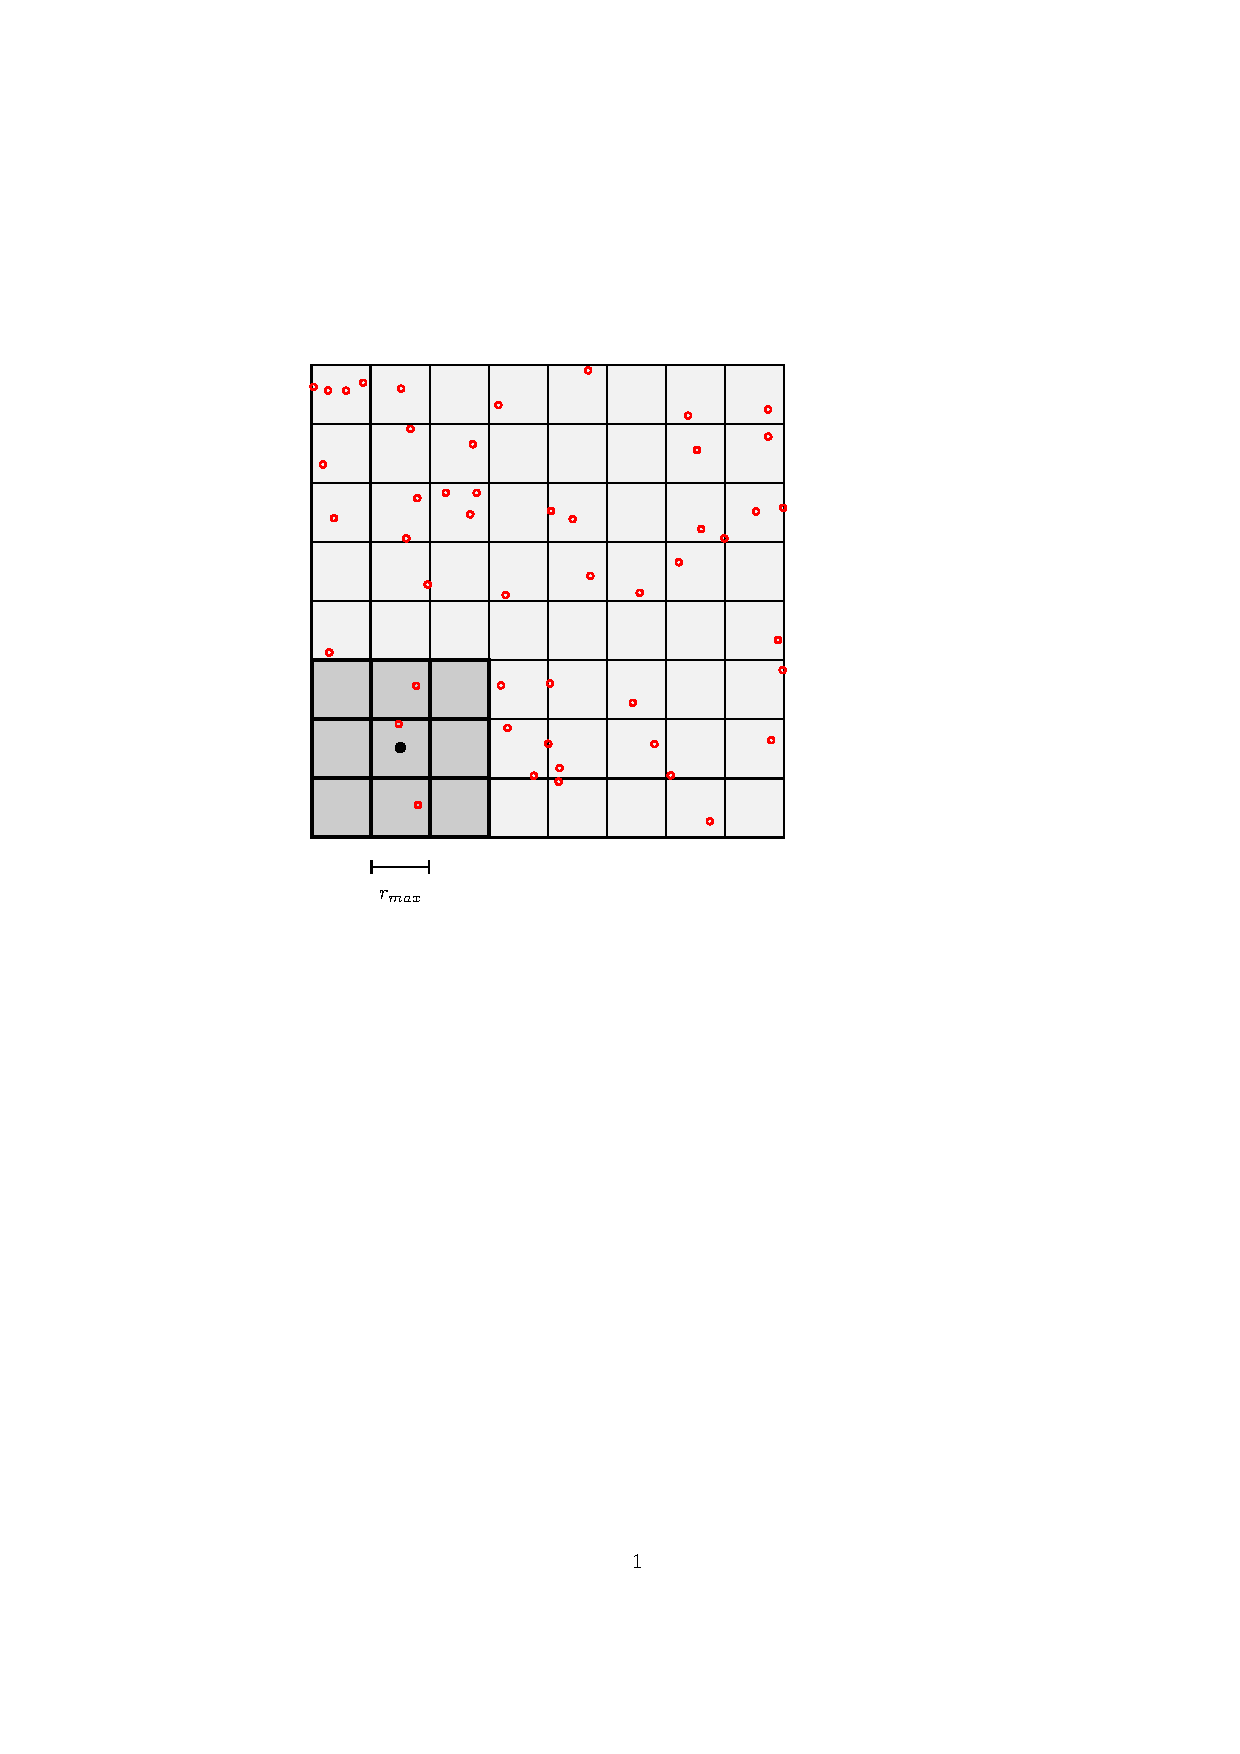
\includegraphics[width=\textwidth,clip=true]{tikz_grid}
\caption{A 2-D grid showing the bin-lattice partitioning scheme. The bigger square show the entire
domain, the red circles show a random distribution of 100 particles. Let's say we want to compute all pairs
for the target blue point, then we would only have to consider red points that are within one cell (the dark shaded region).
A circle with radius \rmax is also drawn to shown the actual pairs that will eventually count in the correlation function.}
\label{fig:grid}
\end{figure}


\subsection{How to Maintain Cache Locality within the Grid}
For all pairs around a given target galaxy, we need to compute distances to all points within all neighbouring 3-d cells.
We ensure that the particle locations are contiguous by moving them into the following \texttt{C struct} in the order in which they arrive.

\begin{lstlisting}[language=C,numbers=none,label={code:celldefn},caption={Definition of the cellarray structure. This 
structure contains the \texttt{X/Y/Z} positions of all the particles that are in one 3-D cell. }]
typedef struct{
  DOUBLE *x;
  DOUBLE *y;
  DOUBLE *z;
  int64_t nelements;
} cellarray;
\end{lstlisting}

\stdsection{Calling the C Libraries}
All of the correlation function codes create a corresponding \texttt{static} library rather than a \texttt{dynamic/shared} library. This was a design decision intended 
to minimize path-issues for the end-user. After the libraries have been created, it is fairly straightforward to use them in an external \texttt{C/python} code. 
\subsection{C bindings}
The \texttt{examples} contains the files \texttt{run\_correlations.c} that shows how to use the three types of correlation function libraries from C. Essentially, the process 
consists of including the appropriate header file and passing the appropriate arrays in the functions. 

\subsubsection{API for \texorpdfstring{\xir}{xi(r)}}
\begin{lstlisting}[language=C,numbers=none,label={code:API_DD},basicstyle=\scriptsize]
typedef struct{
  uint64_t *npairs;
  DOUBLE *rupp;
  DOUBLE *rpavg;
  int nbin;
} results_countpairs;

results_countpairs * countpairs(
const int64_t ND1, const DOUBLE * const X1, const DOUBLE * const Y1, const DOUBLE  * const Z1,
const int64_t ND2, const DOUBLE * const X2, const DOUBLE * const Y2, const DOUBLE  * const Z2,
#ifdef USE_OMP
const int numthreads,
#endif
const int autocorr,
const char *binfile) __attribute__((warn_unused_result));

void free_results(results_countpairs **results);
\end{lstlisting}

\subsubsection{API for \texorpdfstring{\xirppi}{xi(rp,pi)}}
\begin{lstlisting}[language=C,numbers=none,label={code:API_DDrppi},basicstyle=\scriptsize]
typedef struct{
  uint64_t *npairs;
  DOUBLE *rupp;
  DOUBLE *rpavg;
  DOUBLE pimax;
  int nbin;
  int npibin;
} results_countpairs_rp_pi;

results_countpairs_rp_pi * countpairs_rp_pi(
const int64_t ND1, const DOUBLE *X1, const DOUBLE *Y1, const DOUBLE *Z1,
const int64_t ND2, const DOUBLE *X2, const DOUBLE *Y2, const DOUBLE *Z2,
#ifdef USE_OMP
const int numthreads,
#endif
const int autocorr,
const char *binfile,
const double pimax)  __attribute__((warn_unused_result));

void free_results_rp_pi(results_countpairs_rp_pi **results);
\end{lstlisting}

\subsubsection{API for \texorpdfstring{\wprp}{wp(rp)}}
\begin{lstlisting}[language=C,numbers=none,label={code:API_wp},basicstyle=\scriptsize]
typedef struct{
  uint64_t *npairs;
  DOUBLE *wp;
  DOUBLE *rupp;
  DOUBLE *rpavg;
  DOUBLE pimax;
  int nbin;
} results_countpairs_wp;

results_countpairs_wp *countpairs_wp(
const int64_t ND1, DOUBLE * restrict X1, DOUBLE * restrict Y1, DOUBLE * restrict Z1,
const double boxsize, 
#ifdef USE_OMP
const int numthreads,
#endif
const char *binfile,
const double pimax) __attribute__((warn_unused_result));


void free_results_wp(results_countpairs_wp **results);
\end{lstlisting}


\subsection{Python Bindings}
The \texttt{python\_bindings} directory contains python bindings for python 2.x. Note that python3 is not supported out of the box\footnote{In the future, I might switch to 
cython to cover both python2 and python3}. If all went well, then typing \texttt{python call\_correlation\_functions.py} should run the example python code. If you get 
an error (and you are on a MAC), then refer to Section~\ref{section:mac} or the FAQ. 

If you edit the \texttt{common.mk} file and compile for \texttt{double precision} arithmetic, then be sure to change the line:
\begin{lstlisting}[language=python,numbers=none]
dtype=np.float32
\end{lstlisting}
to 
\begin{lstlisting}[language=python,numbers=none]
dtype=np.float64.
\end{lstlisting}
Otherwise, you will get a \texttt{TypeError} at runtime. 


\stdsection{Extending the Code}
\subsection{Different Type of Input Data File}
All of the codes use \texttt{io.c} in the \texttt{io} sub-directory to read-in the data. If you want to specify a different file format, the easiest way would be to edit 
\texttt{io.c}. Decide on the file format code and add another \texttt{strncmp} case in \texttt{io.c}. Remember that the \texttt{x/y/z} are declared as \texttt{void} pointers, 
so you can not directly reference the \texttt{x/y/z} pointers. If you do add support for a different file-type, please submit a pull request and I will be happy to merge it into the 
code-base. 

\subsection{Computing a different type of correlation function}
Let's say, you want to compute a marked correlation function. Now, you will need to read-in/create the marks for each individual point. And then you will have to add an 
appropriate field to the \texttt{cellarray} structure (see \ref{code:celldefn}). 

\subsection{Using SSE instead of AVX}
If your CPU is too old and does not support AVX, then you can still use SSE instrinsics to compute the correlation functions. However, this will require replacing all of the 
AVX sections with corresponding SSE intrinsics. \href{mailto:manodeep@gmail.com}{Email me} and I will guide you through the conversion process. 

%% \bibliographystyle{apj}
%% \bibliography{master}

\end{document}




